% Generated by thesis/ch7/exp2/networks.py -- do not edit by hand.
\begin{sidewaysfigure}
  \centering
  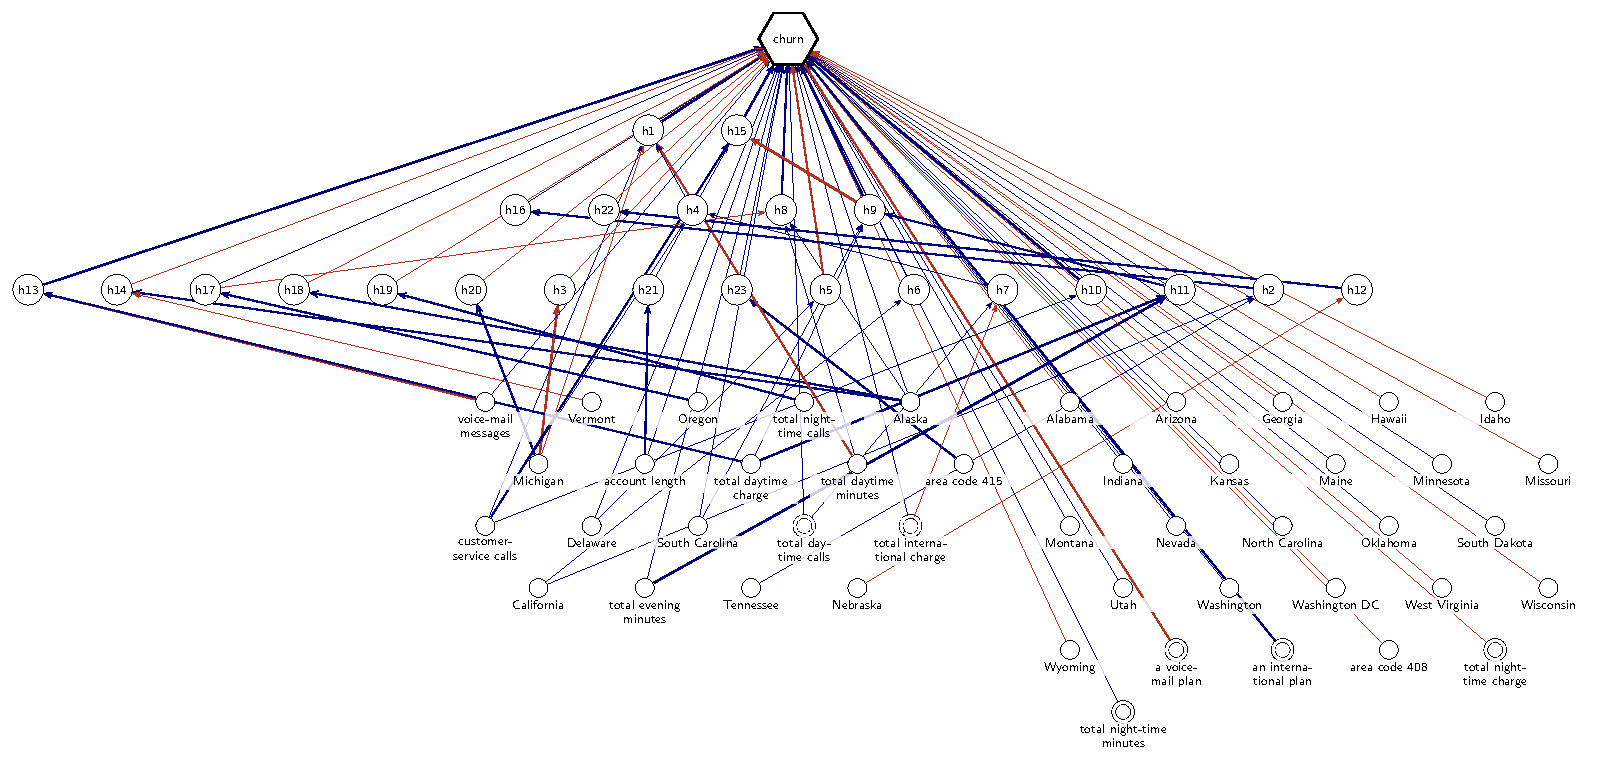
\includegraphics[width=\textheight,height=0.78\textwidth,keepaspectratio]{figures/exp2/networks/churn100-s0-raw}
  \caption{Churn, seed 0 (churn100-s0): the network as trained, before any explanation, in full. Inputs at the bottom (every input column its own node), hidden units by depth, the output at the top; 45 of 71 input columns are connected, with 23 hidden units and 89 enabled connections. Blue: positive weight (raises the score); red: negative weight (lowers it); thicker: larger weight. Orange outline and up arrow: raises the final prediction; teal and down arrow: lowers it; grey and double arrow: depends. Not used (no connection; 26 columns): Iowa, Illinois, Kentucky, Louisiana, Massachusetts, Arkansas, Maryland, Mississippi, North Dakota, New Hampshire, New Jersey, New Mexico, New York, Ohio, Pennsylvania, Rhode Island, Texas, Virginia, Colorado, Connecticut, Florida, area code 510, total evening calls, total evening charge, total international minutes and total international calls.}
  \label{fig:exp2-net-churn100-s0-raw}
\end{sidewaysfigure}
